\documentclass[aspectratio=169,10pt]{beamer}

\usepackage{fontspec}
\usepackage{amsmath,amssymb,bm,mathtools}
\usepackage{booktabs,tabularx,array}
\usepackage{graphicx}
\usepackage{tikz}
\usetikzlibrary{arrows.meta,positioning,shapes.geometric,calc}

\setmainfont{TeX Gyre Pagella}
\setsansfont{TeX Gyre Heros}
\setmonofont{Latin Modern Mono}
\usefonttheme{professionalfonts}

\definecolor{navy}{HTML}{183A5A}
\definecolor{teal}{HTML}{087E8B}
\definecolor{orange}{HTML}{E07A3F}
\definecolor{green}{HTML}{3E8E63}
\definecolor{red}{HTML}{B94A48}
\definecolor{ink}{HTML}{27323A}
\definecolor{muted}{HTML}{65727C}

\setbeamercolor{normal text}{fg=ink,bg=white}
\setbeamercolor{structure}{fg=teal}
\setbeamercolor{frametitle}{fg=navy,bg=white}
\setbeamercolor{title}{fg=navy}
\setbeamercolor{subtitle}{fg=muted}
\setbeamercolor{block title}{fg=white,bg=teal}
\setbeamercolor{block body}{fg=ink,bg=teal!6}
\setbeamercolor{alerted text}{fg=orange}
\setbeamercolor{itemize item}{fg=teal}
\setbeamercolor{itemize subitem}{fg=orange}

\setbeamertemplate{navigation symbols}{}
\setbeamertemplate{itemize item}{\raise0.15ex\hbox{\scriptsize$\blacktriangleright$}}
\setbeamertemplate{itemize subitem}{\raise0.15ex\hbox{\tiny$\blacktriangleright$}}
\setbeamertemplate{frametitle}{%
  \vspace{0.3em}\insertframetitle\par
  \vspace{-0.35em}{\color{teal}\rule{\textwidth}{0.7pt}}
}
\setbeamertemplate{footline}{%
  \leavevmode
  \hbox{%
    \begin{beamercolorbox}[wd=.78\paperwidth,ht=2.7ex,dp=1.1ex,leftskip=1em]{author in head/foot}%
      \color{muted}\scriptsize Accurate Hartree meshes across SCF iterations
    \end{beamercolorbox}%
    \begin{beamercolorbox}[wd=.22\paperwidth,ht=2.7ex,dp=1.1ex,rightskip=1em plus1fil]{date in head/foot}%
      \color{muted}\scriptsize \insertframenumber/\inserttotalframenumber
    \end{beamercolorbox}%
  }
}

\newcommand{\norm}[1]{\left\lVert #1\right\rVert}
\newcommand{\mesh}{\mathcal T}

\title{One Hartree Mesh, Many SCF Iterations}
\subtitle{Accuracy-controlled reuse with a budget of 4--5 mesh updates}
\author{Research proposal}
\date{September 2026}
\begin{document}
\begin{frame}[plain]
\titlepage
\begin{center}\color{teal}\large Build each mesh for a range of densities,\\not just the current density.\end{center}
\end{frame}

\begin{frame}{The research objective}
\begin{block}{A bounded number of mesh changes}
For one fixed-nuclei KS solve, allow at most $B\in\{4,5\}$ accepted Hartree mesh updates after the initial construction. Recompute the Hartree potential at every SCF iteration.
\end{block}
\begin{itemize}
\item An update means a change in connectivity or vertex positions; both invalidate geometry-dependent caches.
\item Within one mesh epoch, keep geometry fixed for many density updates.
\item Each accepted mesh must satisfy a stated Hartree accuracy target and geometric quality conditions.
\end{itemize}
\small\color{muted}Counting convention: $B$ updates means at most $B+1$ accepted meshes. If initial construction counts toward the budget, use $B-1$ updates. Mesh-generation passes inside one construction are recorded separately.
\end{frame}

\begin{frame}{Insert the reusable Hartree solver into KS--SCF}
\small
\[
 H[\rho_k]\psi_i=\epsilon_i\psi_i,\qquad
 H[\rho_k]=-\tfrac12\Delta+V_{\rm ext}+V_H[\rho_k]+V_{\rm xc}[\rho_k].
\]
\[
\rho_k\ \longrightarrow\ \boxed{\widetilde V_{H,\mathcal T_j}[\rho_k]}
\ \longrightarrow\ H[\rho_k]\ \longrightarrow\ \rho_k^{\rm out}
\ \longrightarrow\ \text{mixing}\ \longrightarrow\ \rho_{k+1}.
\]
\begin{columns}[T,onlytextwidth]
\column{.48\textwidth}\begin{block}{Reuse during epoch $j$}
Tetrahedra, quadrature geometry, hierarchy, near/far lists, singular-integration geometry, and static GPU data.
\end{block}
\column{.48\textwidth}\begin{block}{Refresh every iteration}
Density samples, source weights, leaf and parent multipoles, near/far contributions, Hartree potential and energy.
\end{block}
\end{columns}
\small Fixed source and target geometry is required for list reuse. Changes in target locations or the MAC require corresponding list updates.
\end{frame}

\begin{frame}{Existing evidence supports the direction}
\small Manufactured 20-step density sequence; these are \alert{not self-consistent KS results}.
\medskip
\centering
\begin{tabular}{lrrr}
\toprule
Policy & Mesh updates & Sequence time (s) & Maximum $L^2$ error\\
\midrule
Frozen & 0 & 34.548 & $4.83\times10^{-4}$\\
Every-$h$ & 19 & 8.667 & $6.34\times10^{-5}$\\
Periodic ($H=4$) & 4 & 11.576 & $3.67\times10^{-4}$\\
Residual-$h$ & 4 & 7.222 & $6.06\times10^{-5}$\\
\bottomrule
\end{tabular}
\begin{block}{The missing step}
Four updates happened in this experiment. The current trigger does not enforce a total update budget or certify future-density accuracy.
\end{block}
\raggedright\footnotesize
\texttt{max\_reuse=4} bounds consecutive reuse steps, not total rebuilds.\\
Errors exclude step 0; sequence times exclude common initial setup.\\
\color{muted}Source: \texttt{experiment\_results/mesh\_policy\_summary.md}.
\end{frame}

\begin{frame}{Mesh quality has two distinct meanings}
\begin{columns}[T,onlytextwidth]
\column{.48\textwidth}\begin{block}{Geometric validity}
\begin{itemize}
\item Positive tetrahedron volumes.
\item Controlled aspect ratios / minimum quality.
\item Adequate resolution around nuclei and bonds.
\item Valid cluster bounds and near/far lists.
\end{itemize}
\end{block}
\column{.48\textwidth}\begin{block}{Accuracy for the current density}
\begin{itemize}
\item Source representation is resolved.
\item Near/singular quadrature is accurate.
\item Multipole error meets its budget.
\item Transfer to KS targets is accurate.
\end{itemize}
\end{block}
\end{columns}
\medskip
\alert{Good element shapes alone cannot guarantee an accurate Hartree potential.}
\smallskip
\small A mesh can remain geometrically valid while charge moves into an under-resolved region.
\end{frame}

\begin{frame}{Define the accuracy contract before the update rule}
\small For isolated systems in atomic units, let $K\rho(\bm x)=\int_\Omega\rho(\bm y)/|\bm x-\bm y|\,d\bm y$.
\[
\|V_H[\rho_k]-\widetilde V_{H,\mathcal T_j}[\rho_k]\|_X
\le E_{\rm domain}+E_{\rm source}+E_{\rm quad}
+E_{\rm tree}+E_{\rm transfer}\le\tau_k.
\]
\begin{itemize}
\item Choose a norm $X$ relevant to KS assembly; bounds below use $L^\infty$ over the computational domain.
\item Allocate tolerances to each error component. Tightening multipoles cannot repair an under-resolved density.
\item Hold the orbital discretization error to a separate tolerance.
\end{itemize}
\begin{block}{A useful consequence at fixed density}
If $\rho\ge0$, $\int\rho=N_e$, and $\|\delta V_H\|_\infty\le\tau$, then
$|\delta E_H|=|\tfrac12\int\rho\,\delta V_H|\le N_e\tau/2$.
\end{block}
\footnotesize This is a Hartree evaluation bound at fixed density, not a bound on the full self-consistent total-energy error.
\end{frame}

\begin{frame}{Build a mesh for a density family}
\small At rebuild iteration $k_j$, retain several representative densities and increments:
\[
\mathcal S_j=\{\rho_{k_j},\rho_{k_j-1},\ldots\}
\quad\text{and}\quad d_k=\rho_k-\rho_{k-1}.
\]
\begin{enumerate}
\item Evaluate local source indicators on all selected snapshots; include initial atomic densities and bond regions.
\item Mark the union of poorly resolved regions and add a spatial buffer where recent changes are large.
\item Refine until each snapshot passes a stricter mesh tolerance $\gamma\tau_{\rm mesh}$, with $0<\gamma<1$.
\item Coarsen only where every retained snapshot remains resolved; check shapes, charge transfer, and potential accuracy.
\end{enumerate}
\begin{block}{Proposed contribution}
Use a reusable density-family mesh with explicit accuracy headroom and a finite update budget.
\end{block}
\footnotesize Snapshot coverage is a practical design heuristic. It becomes a future-density guarantee only with a bound on densities outside the snapshot family.
\end{frame}

\begin{frame}{A conditional guarantee for many future evaluations}
\small Let $P_j$ be a fixed linear density projection on mesh $\mathcal T_j$ and
$A_j=K(I-P_j)$. Suppose a validated mesh certificate gives
\[
\|A_j\rho_{k_j}\|_\infty\le e_j,\qquad
\|A_j\delta\rho\|_\infty\le C_j\|\delta\rho\|_2.
\]
Then, for every later density with $\|\rho_k-\rho_{k_j}\|_2\le R_j$,
\[
\boxed{\|K\rho_k-KP_j\rho_k\|_\infty\le e_j+C_jR_j.}
\]
\begin{block}{Accuracy headroom becomes a reuse radius}
If $e_j<\tau_{\rm mesh}$ and $C_j>0$, choose
$R_j\le(\tau_{\rm mesh}-e_j)/C_j$.
The mesh remains certified while the density stays within this radius.
\end{block}
\footnotesize This follows from linearity and the triangle inequality. It is conditional on certified constants and source representation; the existing implementation does not yet supply this certificate. Other Hartree error terms must also pass.
\end{frame}

\begin{frame}{What is needed to make the certificate rigorous?}
\small On a bounded domain of diameter $D$, for $\bm x\in\Omega$,
\[
\int_\Omega |\bm x-\bm y|^{-2}\,d\bm y\le4\pi D,
\qquad \|Kf\|_\infty\le\sqrt{4\pi D}\,\|f\|_2.
\]
Hence one safe bound is
\[
 C_j\le\sqrt{4\pi D}\,\|I-P_j\|_{2\to2}.
\]
\begin{itemize}
\item For an $L^2$-orthogonal projection, $\|I-P_j\|_{2\to2}\le1$; the global bound can be very conservative.
\item Obtain sharper local bounds using certified cellwise source errors and kernel integrals.
\item A sampled source residual or a two-resolution difference is an indicator unless its reliability is established.
\item Bound density tails outside $\Omega$ and verify quadrature, multipoles, and transfer separately.
\end{itemize}
\footnotesize These bounds are derived here for the free-space Coulomb kernel. Periodic electrostatics needs a different treatment.
\end{frame}

\begin{frame}{Practical monitoring before full certification}
\small The code currently uses a source-resolution indicator:
\[
\eta_\rho^2=
\frac{\sum_{T\in\mathcal T_j}h_T^2\|\rho-\bar\rho_T\|_{L^2(T)}^2}
{\|\rho\|_{L^2(\Omega)}^2}.
\]
\begin{itemize}
\item Track local indicators and drift from the \emph{epoch anchor} $\rho_{k_j}$; successive small changes can accumulate.
\item Compare selected potentials against enriched quadrature / higher multipole order to diagnose evaluation error.
\item Use independent spatial probes or an enriched source representation to expose missed density features.
\item Monitor electron count, Hartree energy, and the unmixed SCF residual.
\end{itemize}
\begin{block}{Label the evidence correctly}
These checks support an empirical accuracy claim. Finite probes alone do not certify a global norm; a certified implementation must use reliable upper bounds.
\end{block}
\end{frame}

\begin{frame}{Spend 4--5 updates on accuracy stages}
\small Set $B=5$: allow up to four earlier accepted updates and reserve one for final accuracy. For $B=4$, allow three earlier updates plus the reserve.
\medskip
\centering
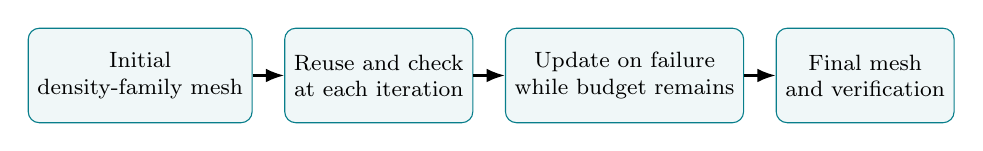
\begin{tikzpicture}[node distance=4mm,box/.style={draw=teal,rounded corners,fill=teal!6,align=center,font=\footnotesize,minimum height=12mm},arr/.style={-{Latex},thick}]
\node[box] (a) {Initial\\density-family mesh};
\node[box,right=of a] (b) {Reuse and check\\at each iteration};
\node[box,right=of b] (c) {Update on failure\\while budget remains};
\node[box,right=of c] (d) {Final mesh\\and verification};
\draw[arr] (a)--(b);\draw[arr] (b)--(c);\draw[arr] (c)--(d);
\end{tikzpicture}
\medskip
\begin{itemize}
\item Use a small number of decreasing tolerance stages ending at $\tau_{\rm final}$.
\item Advance a stage when the unmixed SCF residual is sufficiently small; thresholds require consistent units and calibration.
\item Rebuild only when the active accuracy test fails. Aim below the next stage tolerance to create reuse headroom.
\item If an early failure occurs, spend a remaining update immediately and merge later planned stages.
\end{itemize}
\footnotesize Residual-dependent accuracy is inspired by inexact nonlinear solves; it is not by itself a convergence theorem for mixed KS--SCF.
\end{frame}

\begin{frame}{Budget-aware SCF controller: proposed algorithm}
\small
\begin{enumerate}
\item Construct and verify $\mathcal T_0$; set accepted-update counter $b=0$.
\item At iteration $k$, sample $\rho_k$, check the mesh accuracy, and check the remaining Hartree error components.
\item If evaluation error dominates, increase quadrature/order or tighten the MAC; rebuild affected caches and record that cost.
\item If mesh accuracy fails and $b<B$, construct a density-family mesh with headroom, verify it, accept it, and increment $b$.
\item If accuracy still fails at $b=B$, report \alert{budget/tolerance infeasible}; do not declare a certified solution.
\item On a passing mesh, refresh moments and $V_H$, solve KS, form $\rho_k^{\rm out}$, and mix.
\item Stop only when SCF convergence and the final Hartree accuracy test both pass.
\end{enumerate}
\footnotesize Refinement passes during construction need their own work limit. A fixed mesh-update count does not bound total setup cost or guarantee SCF convergence.
\end{frame}

\begin{frame}{A strict cap requires an explicit feasibility condition}
\begin{block}{Sufficient condition for successful bounded reuse}
The SCF density trajectory can be covered, in iteration order, by at most $B+1$ certified mesh epochs, each meeting the required tolerance over its density family.
\end{block}
\begin{itemize}
\item Arbitrary future charge localization can violate any mesh designed from a few past densities.
\item The final mesh needs enough resolution for the remaining density trajectory at $\tau_{\rm final}$.
\item A more conservative initial/final mesh can reduce updates but increase every potential evaluation cost.
\end{itemize}
\medskip
\alert{The update cap is enforceable. Accuracy within that cap is conditional on mesh capacity and density evolution.}
\end{frame}

\begin{frame}{KS coupling and final acceptance}
\small
\begin{itemize}
\item Evaluate the density on Hartree source points consistently with the orbital representation; verify $\int\rho=N_e$.
\item Evaluate or transfer $V_H$ at the actual KS assembly points. The current leaf-barycenter test is insufficient for this interface.
\item Keep orbital and Hartree meshes separate initially; check transfer error with independent refinement.
\item After a mesh change, reevaluate the current density's potential. Reset or consistently transform mixing history if its representation changes.
\item Before acceptance, use $\tau_{\rm final}$ and recompute the unmixed residual with the accurate Hamiltonian; continue SCF if needed.
\end{itemize}
\begin{block}{Why the last check matters}
Convergence on a coarse Hartree mesh can be convergence to a perturbed discrete problem. Final verification must test the intended accuracy.
\end{block}
\end{frame}

\begin{frame}{Experiments that would establish the new idea}
\small
\begin{tabularx}{\textwidth}{lX}
\toprule
Comparison & What it tests\\\midrule
Every-step adaptation & Accuracy and full-time reference\\
Frozen initial mesh & Whether initial mesh quality is sufficient\\
Budgeted current-density mesh & Value of the update controller alone\\
Budgeted density-family mesh & Value of preparing for future densities\\
\bottomrule
\end{tabularx}
\medskip
\begin{itemize}
\item First replay identical stored KS density sequences through all policies; then run fully coupled SCF comparisons.
\item Test several initial guesses, charge redistribution, and oscillatory trajectories; include budget-exhaustion cases.
\item Report accepted mesh updates, internal refinement passes, cache rebuilds, peak mesh size, checking cost, and total SCF wall time.
\item Compare maximum Hartree error, final total energy, density, SCF iterations, and failures against a converged reference.
\end{itemize}
\alert{Success: target accuracy and SCF convergence with $b\le4$ or $5$, at lower total cost.}
\end{frame}

\begin{frame}{Discussion: what is new, and what remains to prove?}
\begin{block}{Working research statement}
Construct each adaptive Hartree mesh for a controlled family of SCF densities, monitor its validity during reuse, and allocate at most 4--5 accepted mesh updates across the solve.
\end{block}
\begin{itemize}
\item Existing evidence: four residual-driven updates work well on one manufactured sequence.
\item Proposed mechanism: density-family adaptation, accuracy headroom, epoch-anchor drift, and a reserved final update.
\item Mathematical task: reliable source/evaluation bounds and assumptions that cover the remaining density trajectory.
\item Numerical task: show that extra mesh preparation and checking cost less than repeated rebuilding in actual KS--SCF.
\end{itemize}
\end{frame}

\begin{frame}{Sources and scope}
\footnotesize
\begin{itemize}
\item Local implementation: \texttt{compare\_mesh\_modes.cpp}; policies and indicator documented in \texttt{mesh\_modes.md}.
\item Local measurements: \texttt{experiment\_results/mesh\_policy\_summary.md}; manufactured density sequence, 20 steps.
\item Chen et al., \emph{Adaptive Finite Element Approximations for Kohn--Sham Models}. \href{https://arxiv.org/abs/1302.6896}{arXiv:1302.6896}. Residual-based adaptation and convergence analysis for KS finite elements; not a certificate for this integral treecode.
\item Dembo, Eisenstat, Steihaug, \emph{Inexact Newton Methods}, SIAM J. Numer. Anal. 19 (1982), 400--408. \href{https://doi.org/10.1137/0719025}{doi:10.1137/0719025}. Motivation for matching inner accuracy to nonlinear progress; the SCF controller here is a proposal.
\end{itemize}
\medskip
The density-family strategy, update-budget controller, and conditional reuse bound in this deck are proposed work. No new KS experiment or certified estimator is claimed.
\end{frame}
\end{document}
